%%%%%%%%%%%%%%%%%%%%%%%%%%%%%%%%%%%%%%%%%
% Programming/Coding Assignment
% LaTeX Template
%
% This template has been downloaded from:
% http://www.latextemplates.com
%
% Original author:
% Ted Pavlic (http://www.tedpavlic.com)
%
% Note:
% The \lipsum[#] commands throughout this template generate dummy text
% to fill the template out. These commands should all be removed when 
% writing assignment content.
%
% This template uses a Perl script as an example snippet of code, most other
% languages are also usable. Configure them in the "CODE INCLUSION 
% CONFIGURATION" section.
%
%%%%%%%%%%%%%%%%%%%%%%%%%%%%%%%%%%%%%%%%%

%----------------------------------------------------------------------------------------
%	PACKAGES AND OTHER DOCUMENT CONFIGURATIONS
%----------------------------------------------------------------------------------------

\documentclass{article}

\usepackage{fancyhdr} % Required for custom headers
\usepackage{lastpage} % Required to determine the last page for the footer
\usepackage{extramarks} % Required for headers and footers
\usepackage[usenames,dvipsnames]{color} % Required for custom colors
\usepackage{graphicx} % Required to insert images
\usepackage{listings} % Required for insertion of code
\usepackage{courier} % Required for the courier font
\usepackage{float}



% Margins
\topmargin=-0.45in
\evensidemargin=0in
\oddsidemargin=0in
\textwidth=6.5in
\textheight=9.0in
\headsep=0.25in

\linespread{1.1} % Line spacing

% Set up the header and footer
\pagestyle{fancy}
\lhead{\hmwkAuthorName} % Top left header
\chead{\hmwkClass\ (\hmwkClassInstructor\ \hmwkClassTime): \hmwkTitle} % Top center head
\rhead{\firstxmark} % Top right header
\lfoot{\lastxmark} % Bottom left footer
\cfoot{} % Bottom center footer
\rfoot{Page\ \thepage\ of\ \protect\pageref{LastPage}} % Bottom right footer
\renewcommand\headrulewidth{0.4pt} % Size of the header rule
\renewcommand\footrulewidth{0.4pt} % Size of the footer rule

\setlength\parindent{0pt} % Removes all indentation from paragraphs

%----------------------------------------------------------------------------------------
%	CODE INCLUSION CONFIGURATION
%----------------------------------------------------------------------------------------

\definecolor{MyDarkGreen}{rgb}{0.0,0.4,0.0} % This is the color used for comments
\lstloadlanguages{Python} % Load Perl syntax for listings, for a list of other languages supported see: ftp://ftp.tex.ac.uk/tex-archive/macros/latex/contrib/listings/listings.pdf
\lstset{language=Python, % Use Perl in this example
        frame=single, % Single frame around code
        basicstyle=\small\ttfamily, % Use small true type font
        keywordstyle=[1]\color{Blue}\bf, % Perl functions bold and blue
        keywordstyle=[2]\color{Purple}, % Perl function arguments purple
        keywordstyle=[3]\color{Blue}\underbar, % Custom functions underlined and blue
        identifierstyle=, % Nothing special about identifiers                                         
        commentstyle=\usefont{T1}{pcr}{m}{sl}\color{MyDarkGreen}\small, % Comments small dark green courier font
        stringstyle=\color{Purple}, % Strings are purple
        showstringspaces=false, % Don't put marks in string spaces
        tabsize=5, % 5 spaces per tab
        %
        % Put standard Perl functions not included in the default language here
        morekeywords={rand},
        %
        % Put Perl function parameters here
        morekeywords=[2]{on, off, interp},
        %
        % Put user defined functions here
        morekeywords=[3]{test},
       	%
        morecomment=[l][\color{Blue}]{...}, % Line continuation (...) like blue comment
        numbers=left, % Line numbers on left
        firstnumber=1, % Line numbers start with line 1
        numberstyle=\tiny\color{Blue}, % Line numbers are blue and small
        stepnumber=5 % Line numbers go in steps of 5
}

% Creates a new command to include a perl script, the first parameter is the filename of the script (without .pl), the second parameter is the caption
\newcommand{\python}[2]{
\begin{itemize}
\item[]\lstinputlisting[caption=#2,label=#1]{#1.pl}
\end{itemize}
}

%----------------------------------------------------------------------------------------
%	DOCUMENT STRUCTURE COMMANDS
%	Skip this unless you know what you're doing
%----------------------------------------------------------------------------------------

% Header and footer for when a page split occurs within a problem environment
\newcommand{\enterProblemHeader}[1]{
\nobreak\extramarks{#1}{#1 continued on next page\ldots}\nobreak
\nobreak\extramarks{#1 (continued)}{#1 continued on next page\ldots}\nobreak
}

% Header and footer for when a page split occurs between problem environments
\newcommand{\exitProblemHeader}[1]{
\nobreak\extramarks{#1 (continued)}{#1 continued on next page\ldots}\nobreak
\nobreak\extramarks{#1}{}\nobreak
}

\setcounter{secnumdepth}{0} % Removes default section numbers
\newcounter{homeworkProblemCounter} % Creates a counter to keep track of the number of problems

\newcommand{\homeworkProblemName}{}
\newenvironment{homeworkProblem}[1][Problem \arabic{homeworkProblemCounter}]{ % Makes a new environment called homeworkProblem which takes 1 argument (custom name) but the default is "Problem #"
\stepcounter{homeworkProblemCounter} % Increase counter for number of problems
\renewcommand{\homeworkProblemName}{#1} % Assign \homeworkProblemName the name of the problem
\section{\homeworkProblemName} % Make a section in the document with the custom problem count
\enterProblemHeader{\homeworkProblemName} % Header and footer within the environment
}{
\exitProblemHeader{\homeworkProblemName} % Header and footer after the environment
}

\newcommand{\problemAnswer}[1]{ % Defines the problem answer command with the content as the only argument
\noindent\framebox[\columnwidth][c]{\begin{minipage}{0.98\columnwidth}#1\end{minipage}} % Makes the box around the problem answer and puts the content inside
}

\newcommand{\homeworkSectionName}{}
\newenvironment{homeworkSection}[1]{ % New environment for sections within homework problems, takes 1 argument - the name of the section
\renewcommand{\homeworkSectionName}{#1} % Assign \homeworkSectionName to the name of the section from the environment argument
\subsection{\homeworkSectionName} % Make a subsection with the custom name of the subsection
\enterProblemHeader{\homeworkProblemName\ [\homeworkSectionName]} % Header and footer within the environment
}{
\enterProblemHeader{\homeworkProblemName} % Header and footer after the environment
}

%----------------------------------------------------------------------------------------
%	NAME AND CLASS SECTION
%----------------------------------------------------------------------------------------

\newcommand{\hmwkTitle}{Project\ \#1} % Assignment title
\newcommand{\hmwkDueDate}{Tuesday,\ May\ 2,\ 2017} % Due date
\newcommand{\hmwkClass}{PHYSICS\ 188B} % Course/class
\newcommand{\hmwkClassTime}{12:30PM} % Class/lecture time
\newcommand{\hmwkClassInstructor}{Samani} % Teacher/lecturer
\newcommand{\hmwkAuthorName}{Kevin Belleville} % Your name

%----------------------------------------------------------------------------------------
%	TITLE PAGE
%----------------------------------------------------------------------------------------

\title{
\vspace{2in}
\textmd{\textbf{\hmwkClass:\ \hmwkTitle}}\\
\normalsize\vspace{0.1in}\small{Due\ on\ \hmwkDueDate}\\
\vspace{0.1in}\large{\textit{\hmwkClassInstructor\ \hmwkClassTime}}
\vspace{3in}
}

\author{\textbf{\hmwkAuthorName}}
\date{} % Insert date here if you want it to appear below your name

%----------------------------------------------------------------------------------------

\begin{document}

\maketitle

%----------------------------------------------------------------------------------------
%	TABLE OF CONTENTS
%----------------------------------------------------------------------------------------

%\setcounter{tocdepth}{1} % Uncomment this line if you don't want subsections listed in the ToC

\newpage
\tableofcontents
\newpage

%----------------------------------------------------------------------------------------
%	PROBLEM 1
%----------------------------------------------------------------------------------------

% To have just one problem per page, simply put a \clearpage after each problem

\begin{homeworkProblem}

1. \textbf{The one-dimensional harmonic oscillator is described by the equation}

\begin{equation}
\ddot{x}(t) = -\omega^2 x(t), \qquad \omega > 0
\end{equation}

\textbf{a. Determine the general solution to the initial value problem for the harmonic oscillator with initial conditions}

\begin{equation}
x(0) = x_0 \qquad \dot{x}(0) = 0 \qquad x_0 \neq 0
\end{equation}

\textbf{Comment on what the general solution looks like in phase space, and make a few
phase space plots for some fixed $\omega$ and various $x_0$ .} \\


The general solution is:
\begin{equation}
x(t) = A\cos{\omega t} + B\sin{\omega t}
\end{equation}

\begin{equation}
\dot{x}(t) = -A\omega\sin{\omega t} + B\omega\cos{\omega t}
\end{equation}

Substituting the given initial conditions, we can determine the solution:

\begin{equation}
x(0) = x_0 = A\cos{\omega \cdot 0} + B\sin{\omega \cdot 0} 
\end{equation}
\begin{equation}
x_0 = A \cdot 1 + B \cdot 0 
\end{equation}
\begin{equation}
A = x_0
\end{equation}

\begin{equation}
\dot{x}(0) = 0 = -A\omega\sin{\omega \cdot 0} + B\omega\cos{\omega \cdot 0}
\end{equation}
\begin{equation}
0 = -A\omega \cdot 0+ B\omega \cdot 1
\end{equation}
\begin{equation}
B = 0
\end{equation}

And the final solution is:

\begin{equation}
x(t) = x_0\cos{\omega t}
\end{equation} \\

%% phase space plots here

To compare for different initial conditions, I vary the initial value of x while keeping the frequency $\omega$ the same, to show how this affect the phase space plot.

\begin{figure}[H]
\centering
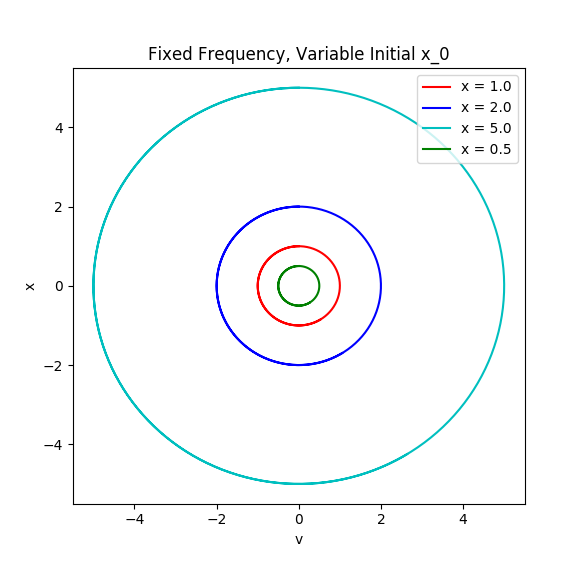
\includegraphics[width=0.75\columnwidth]{part_a.png} % Example image
\caption{We see that changing the initial value of x does not change the nature of the system, (everything is still in a cyclic motion), it just affects where the motion begins.}

\end{figure}




\textbf{b. Write down the Hamiltonian and derive Hamilton's equations for the simple harmonic oscillator of mass $m$ and frequency $\omega$.} \\

The Hamiltonian is defined as:

\begin{equation}
H = T + V
\end{equation}

where $T$ is the kinetic energy and $V$ is the potential. In the case of the simple harmonic oscillator, this equation becomes:

\begin{equation}
H = \frac{p^2}{2m} + \frac{m \omega^2}{2} x^2
\end{equation}

Hamilton's equations are:

\begin{equation}
\dot{q_i} = \frac{\partial H}{\partial p_i}, \qquad \dot{p_i} = -\frac{\partial H}{\partial q_i}
\end{equation}

In our case, the equations become:

\begin{equation}
\dot{x} = \frac{\partial H}{\partial p}, \qquad \dot{p} = -\frac{\partial H}{\partial x}
\end{equation}

\begin{equation}
\dot{x} = \frac{p}{m}, \qquad \dot{p} = -kx
\end{equation} \\ 



\textbf{c. Solve the initial value numerically using Euler’s Method, RK2, RK4, SE1, and
SE2 for various step sizes. Make both plots of the position as a function of time
and phase space plots comparing the numerical solution to the exact solution.
Comment on your results.} \\

First, I will compare the impact of the step size on each method.

\begin{figure}[H]
\centering
\begin{minipage}[b]{0.49\textwidth}
	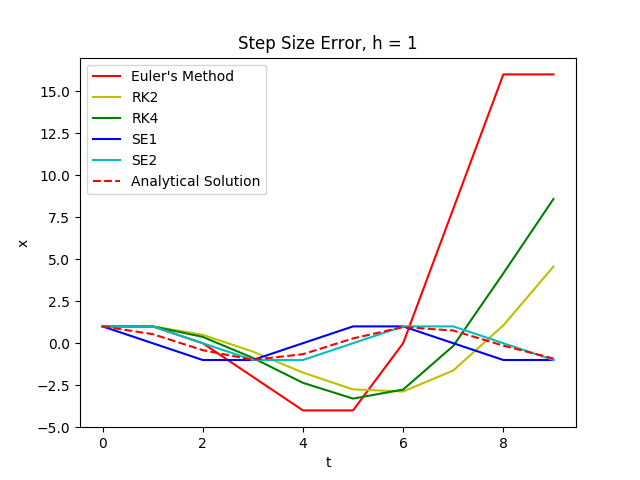
\includegraphics[width=\textwidth]{step_size_1.png}
	\caption{For $h=1$, none of the methods converge to the correct solution. Euler's method, RK2, and RK4 are much further off than the Sympletic methods.}
\end{minipage}
\hfill
\begin{minipage}[b]{0.49\textwidth}
	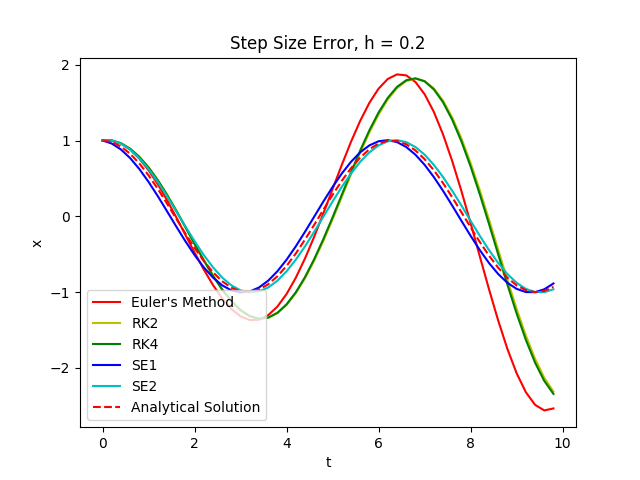
\includegraphics[width=\textwidth]{step_size_3.png}
	\caption{For $h=0.2$, the sympletic methods are beginning to show promise, while the Euler methods are still a ways away.}
\end{minipage}

\centering
\begin{minipage}[b]{0.49\textwidth}
	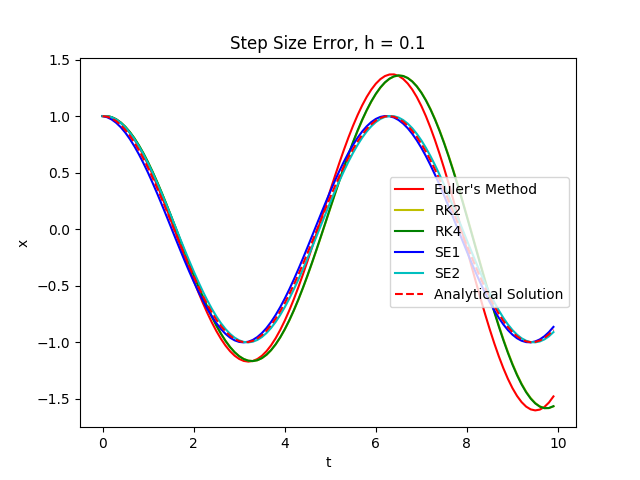
\includegraphics[width=\textwidth]{step_size_4.png}
	\caption{For $h=0.1$, the sympletic methods are already nearly where they need to be (from our view); the Euler methods are making progress, but still not yet acceptable.}
\end{minipage}
\hfill
\begin{minipage}[b]{0.49\textwidth}
	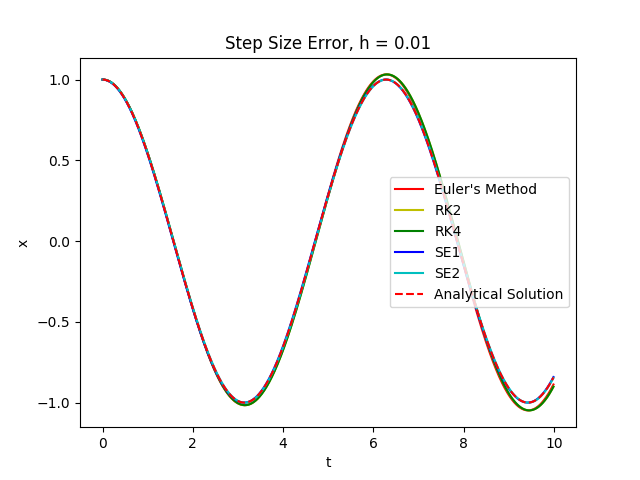
\includegraphics[width=\textwidth]{step_size_5.png}
	\caption{For $h=0.01$, all methods are essentially in line with the analytic solution now. Although all still have errors, they are minute at this step size. This is acceptable.}
\end{minipage}
\end{figure} 

One can notice that the sympletic methods are more correct for smaller step sizes, but all methods need a decently small step size to converge to the analytical solution. However, a small step size means more calculations for the computer, so we must find a compromise between effectiveness of the step size and the time it takes to compute. Next I will compare the effectiveness of each method, by comparing it to the analytical solution. I will first use phase space plots, and then the position versus time plots.

\begin{figure}[H]
\centering
\begin{minipage}[b]{0.49\textwidth}
	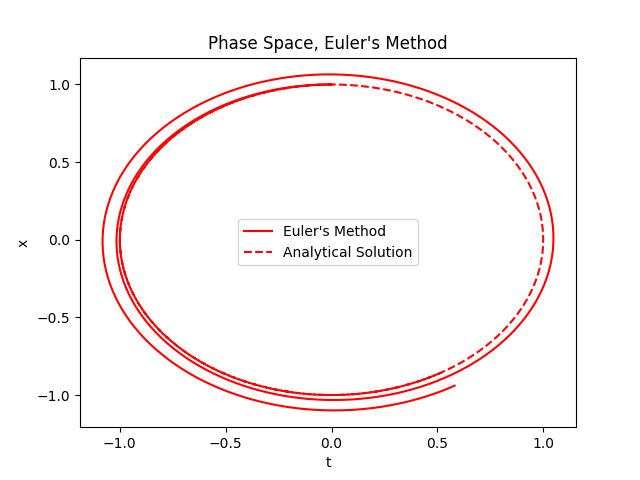
\includegraphics[width=\textwidth]{phase_space_1.png}
	\caption{Euler's Method}
\end{minipage}
\hfill
\begin{minipage}[b]{0.49\textwidth}
	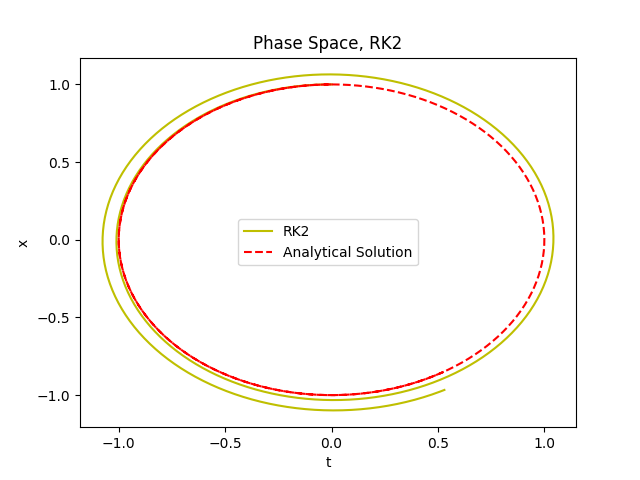
\includegraphics[width=\textwidth]{phase_space_2.png}
	\caption{Runge-Kutta 2}
\end{minipage}

\centering
\begin{minipage}[b]{0.49\textwidth}
	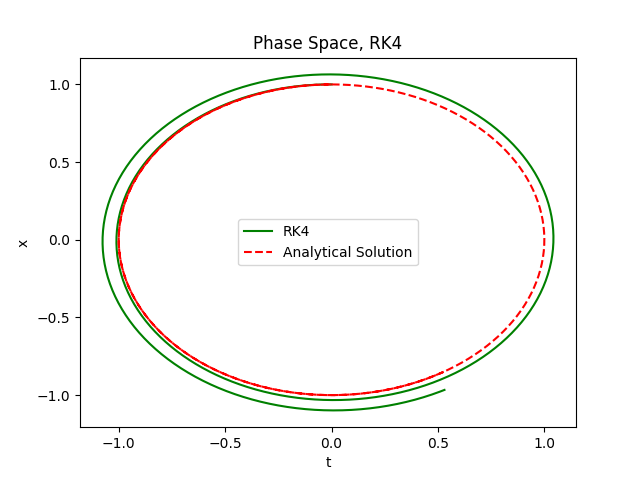
\includegraphics[width=\textwidth]{phase_space_3.png}
	\caption{Runge-Kutta 4}
\end{minipage}
\centering
\begin{minipage}[b]{0.49\textwidth}
	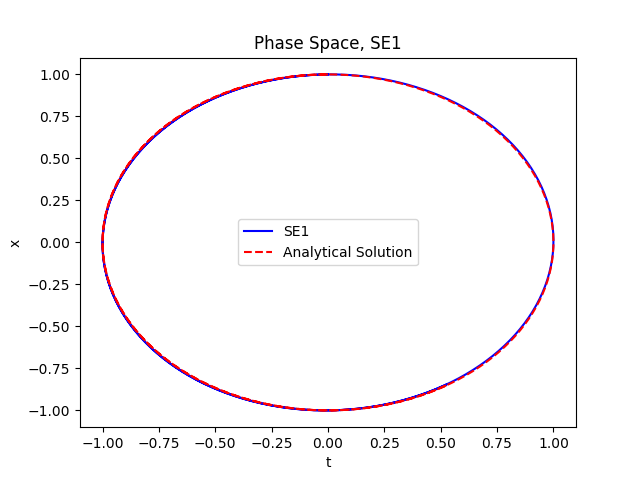
\includegraphics[width=\textwidth]{phase_space_4.png}
	\caption{Sympletic Euler 1}
\end{minipage}
\hfill
\begin{minipage}[b]{0.49\textwidth}
	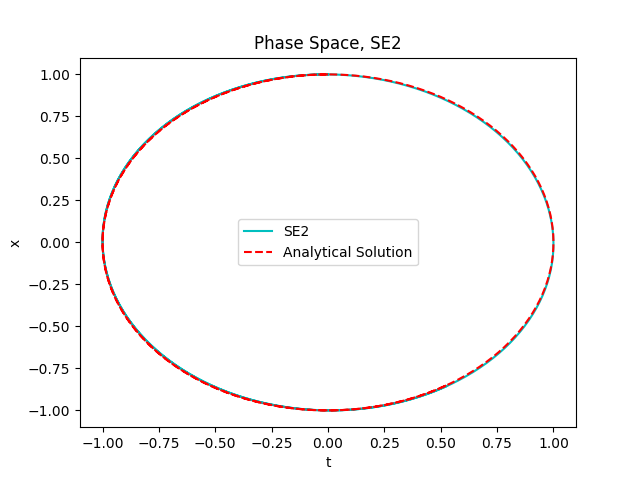
\includegraphics[width=\textwidth]{phase_space_5.png}
	\caption{Sympletic Euler 2}
\end{minipage}

\end{figure} 

Although I could have set the step size extremely small, such that all methods worked very well, I wanted to pick a decently sized step size, so that I could still see the differences between the methods. I settled with a step size of $h=0.02$. In our plots above, we can determine that the sympletic methods are much faster/better to calculate the solutions. Since they are essentially the same method but reverse, it makes sense that they would be nearly exactly the same for sufficiently large step sizes. Euler's method, RK2, and RK4, however, are much worse off than the sympletic methods. At this step size, it seems that the error shaved off by using RK2, or RK4, does not make much off a difference. (But it still makes a difference for smaller step sizes.) Although it does not make much of a difference in our case, it also does not use much more computing power, while still being slightly more accurate, so it should be used anyway.\\



Below, I compare the methods in position plots.

\begin{figure}[H]
\centering
\begin{minipage}[b]{0.49\textwidth}
	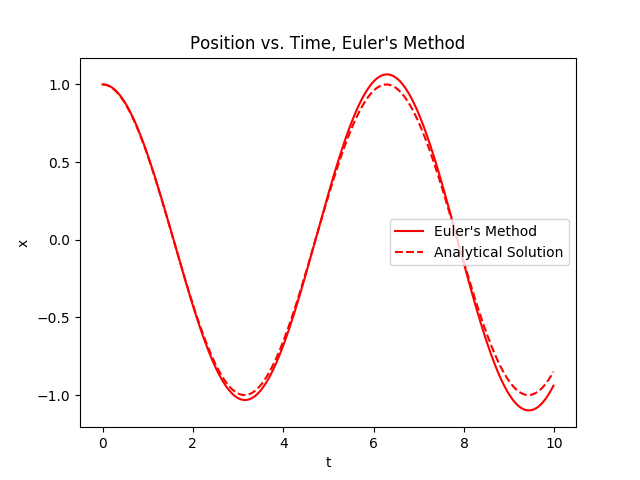
\includegraphics[width=\textwidth]{pos_1.png}
	\caption{Euler's Method}
\end{minipage}
\hfill
\begin{minipage}[b]{0.49\textwidth}
	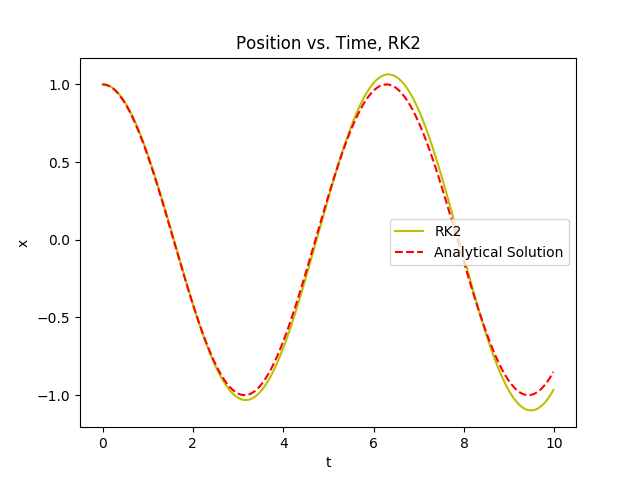
\includegraphics[width=\textwidth]{pos_2.png}
	\caption{Runge-Kutta 2}
\end{minipage}

\centering
\begin{minipage}[b]{0.49\textwidth}
	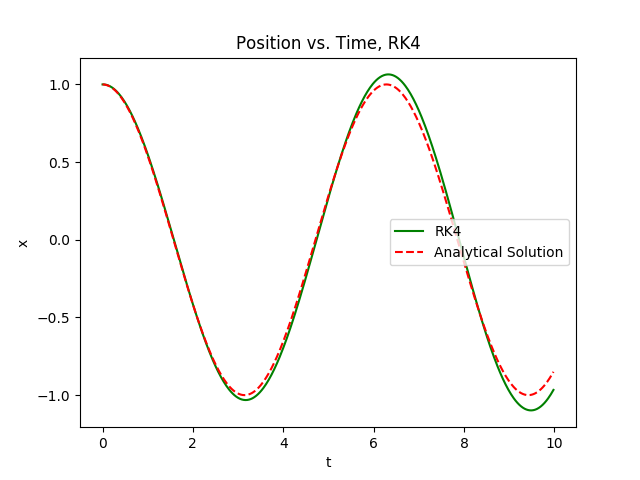
\includegraphics[width=\textwidth]{pos_3.png}
	\caption{Runge-Kutta 4}
\end{minipage}
\centering
\begin{minipage}[b]{0.49\textwidth}
	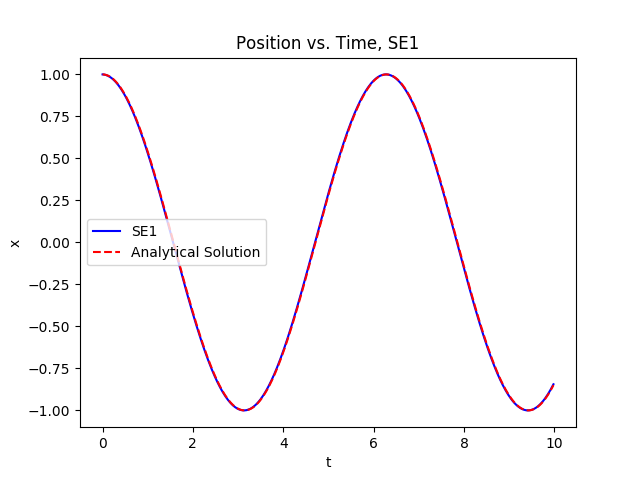
\includegraphics[width=\textwidth]{pos_4.png}
	\caption{Sympletic Euler 1}
\end{minipage}
\end{figure} 

\begin{figure}
\centering
\begin{minipage}[b]{0.49\textwidth}
	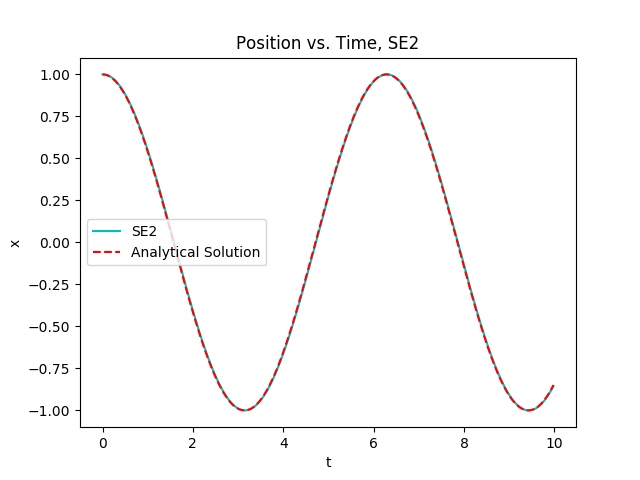
\includegraphics[width=\textwidth]{pos_5.png}
	\caption{Sympletic Euler 2}
\end{minipage}
\end{figure}

In the plots above, we can see the same trends as we have seen previously. SE1 and SE2 are nearly the same, while Euler's method, RK2, and RK4 are less accurate.


\newpage
\textbf{d. Check energy conservation for each solver by graphing total energy (kinetic plus
potential) versus time and comment on your results.} \\

\begin{figure}[H]
\centering
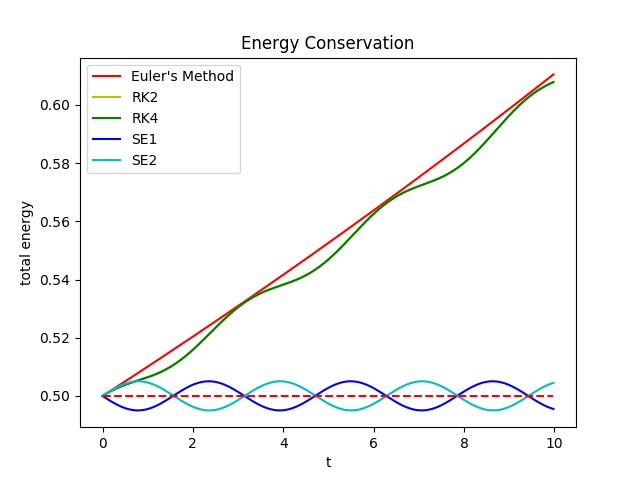
\includegraphics[scale=0.8]{energy.png}
\end{figure}

I calculated the total energy which is just the kinetic energy added to the potential energy for each method. The analytical method obviously conserves energy. Euler's method, RK2, and RK4 all increase gradually over time, but in a significant amount. Euler's increases linearly, but RK2 and RK4 increase in a cyclic way, which I am not sure why it does that. SE1 and SE2 are inverse of each other, but both oscillate around the correct value, which means they will be close to the correct answer as we increase the calculations, unlike the other three methods.


\end{homeworkProblem}

\clearpage

%----------------------------------------------------------------------------------------
%	PROBLEM 2
%----------------------------------------------------------------------------------------

\begin{homeworkProblem}

a. \textbf{Write down the system of equations satisfied by planets ineteracting gravitationally according to Newton's Universal Law of Gravitation (the two-body problem), and show in the standard way that the system of equations can be reduced to that of a single body executing a planar orbit around a fixed force center at the origin.} \\



For a system of two masses $m_1 $ and $m_2$, and their position vectors $\vec{r}_1$ and $\vec{r}_2$, and center-of-mass vector $\vec{R}$, we can determine the equations of motion by simplifying the system from a two-body problem to a signle-body problem. To do this, we define our relative position vector to be $\vec{r} = \vec{r}_1 - \vec{r}_2$, and our center-of-mass vector to be $\vec{R} = 0$ so that the it is the origin of the coordinate system. By doing this, our potential is only a function of $r = |\vec{r}_1 - \vec{r}_2|$. Our Lagrangian is then:

\begin{equation}
L = \frac{1}{2} m_1 | \dot{\vec{r}}_1 | + \frac{1}{2} m_2 | \dot{\vec{r}}_2 | - U(r)
\end{equation}

By setting $\vec{R} = 0$, we then by conservation of momentum have:

\begin{equation}
m_1 \vec{r}_1 + m_1 \vec{r}_1 = 0
\end{equation}

We can utilize our relative position vector $\vec{r}$, and define $\vec{r}_1$ and $\vec{r}_2$ in terms of the masses and itself.

\begin{equation}
\vec{r}_1 = \frac{m_2}{m_1+m_2} \vec{r}
\end{equation}
\begin{equation}
\vec{r}_2 = \frac{m_1}{m_1+m_2} \vec{r}
\end{equation}

We also define a quantity of "reduced mass" as:

\begin{equation}
\mu \equiv \frac{m_1 m_2}{m_1 + m_2}
\end{equation}

Using this new reduced mass, we simplify the Lagrangian into an expression for which there is only a single "body", but is in fact a "particle" of mass $\mu$ in a central field potential $U(r)$:

\begin{equation}
L = \frac{1}{2}\mu | \dot{\vec{r}} |^2 - U(r)
\end{equation}\\




b. \textbf{Show how the reduced two-body problem is solved exactly, and write down explicit expression for the closed orbits.}\\



In planetary motion, there is another independent variable $\theta$ which describes the angle of the planet. The equation above can be adapted to include it as:

\begin{equation}
L = \frac{1}{2}\mu \left( \dot{\vec{r}}^2 + r^2 \dot{\theta}^2 \right) - U(r)
\end{equation}

We can then find two equations of motion, one for $r$ and one for $\theta$. To begin with the $\theta$ component, we deduce with the Lagrangian equation that its first integral of motion is constant:

\begin{equation}
 p_{\theta} \equiv \frac{\partial L}{\partial \dot{\theta}} = \mu r^2 \dot{\theta}
\end{equation}
\begin{equation}
l \equiv \mu r^2 \dot{\theta}
\end{equation}

With this new constant $l$ we can find the total energy of the system:
\begin{equation}
E = \frac{1}{2}\mu \dot{r}^2 + \frac{1}{2} \frac{l^2}{\mu r^2} + U(r)
\end{equation}

Solving for $\dot{r}$, this becomes:
\begin{equation}
\dot{r} = \frac{dr}{dt} = \pm \sqrt{\frac{2}{\mu}\left( E-U \right) - \frac{l^2}{\mu^2 r^2}}
\end{equation}

We can determine $d\theta$ to be:
\begin{equation}
d\theta = \frac{d\theta}{dt}\frac{dt}{dr} dr = \frac{\dot{\theta}}{\dot{r}}
\end{equation}

which with $\dot{\theta} = l/\mu r^2$ can calculate the motion of $\theta$:

\begin{equation}
\theta (r) = \int \frac{\pm (l/r^2) dr}{\sqrt{2\mu \left( E-U-\frac{l^2}{2\mu r^2}\right)}}
\end{equation}

To find the equation of motion for $r$, we start with Lagrange's equation:
\begin{equation}
\frac{\partial L}{\partial r} - \frac{d}{dt} \frac{\partial L}{\partial \dot{r}} = 0
\end{equation}
\begin{equation}
\mu (\ddot{r} - r\dot{\theta}^2 = -\frac{\partial U}{\partial r} = F(r)
\end{equation}

We define $u \equiv \frac{1}{r}$ to make calculations easier, then compute:

\begin{equation}
\frac{du}{d\theta} = -\frac{1}{r^2} \frac{dr}{d\theta} = -\frac{1}{r^2}\frac{\dot{r}}{\dot{\theta}} = - \frac{\mu}{l} \dot{r}
\end{equation}

Then we solve for the second derivative:

\begin{equation}
\frac{d^2 u}{d\theta^2} = \frac{d}{d\theta} \left( -\frac{\mu}{l} \dot{r}\right) = -\frac{\mu}{l\dot{\theta}} \ddot{r}
\end{equation}

Solving for $\ddot{r}$ and $r$:

\begin{equation}
\ddot{r} = - \frac{l^2}{\mu^2} u^2 \frac{d^2 u}{d\theta^2}
\end{equation}
\begin{equation}
r \dot{\theta}^2 = \frac{l^2}{\mu^2} u^3
\end{equation}

Which gives us the equation of motion for $r$:

\begin{equation}
\frac{d^2}{d\theta^2}\left(\frac{1}{r}\right) + \frac{1}{r} = -\frac{\mu r^2}{l^2} F(r)
\end{equation}\\




c. \textbf{Write down the Hamiltonian and the corresponding Hamilton's equations for the reduced two-body problem.}\\


The Hamiltonian can be deduced from the Lagrangian which we already have from before:

\begin{equation}
L = \frac{1}{2}\mu \left( \dot{\vec{r}}^2 + r^2 \dot{\theta}^2 \right) - U(r)
\end{equation}

The momenta of the system for $r$ and $\theta$ is then:

\begin{equation}
p_r = \frac{\partial L}{\partial \dot{r}} = \mu \dot{r}
\end{equation}

\begin{equation}
p_{\theta} = \frac{\partial L}{\partial \dot{\theta}} = \mu r^2 \dot{\theta}
\end{equation}

The Hamiltonian is:

\begin{equation}
H = \dot{r} p_r + \dot{theta} p_{\theta} - L
\end{equation}

Taking $U(r) = -k/r$ for gravitational motion, we solve for H:

\begin{equation}
H = \frac{p^2_r}{2\mu} + \frac{p^2_{\theta}}{2\mu r^2} - \frac{k}{r}
\end{equation}

Hamilton's equations in this case are:

\begin{equation}
\dot{r} = \frac{\partial H}{\partial \theta}
\end{equation}
\begin{equation}
\dot{\theta} = \frac{\partial H}{\partial r}
\end{equation}

Since $\frac{\partial H }{\partial \theta}$ is $0$, $\dot{r} = 0$. For $\dot{\theta}$, however:

\begin{equation}
\mu r \dot{\theta}^2 + \dot{\theta} + \frac{k}{2r^2} = 0
\end{equation}



d. \textbf{Show that Kepler's Second Law (equal areas in equal times) is equivalent to angular momentum conservation.} \\

Recall that:

\begin{equation}
l \equiv \mu r^2 \dot{theta}
\end{equation}

and $l$ is a constant. To calculate an area being swept out between two times, $t_1$ and $t_2$, of an amount $dt$ it's a simple triangle:

\begin{equation}
dA = \frac{1}{2} r^2 d\theta
\end{equation}

If we divide this area by a time interval, the areal velocity (how fast the area changes) is:

\begin{equation}
\frac{dA}{dt} = \frac{1}{2} r^2 \frac{d\theta}{dt} = \frac{1}{2}r^2 \dot{\theta}
\end{equation}

\begin{equation}
 = \frac{l}{2\mu}
\end{equation}

which is a constant. This means that the areal velocity is constant in time, which proves Kepler's Second Law. Kepler's law states that for any given time period, the orbital path of a planet around a sun will fill out a certain amount of area. \\




e. \textbf{Use either SE1 or SE2 to numerically solve the reduced two-body problem for various initial conditions that form closed orbits, and plot the orbits against the corresponding exact orbits.}\\ 



To use the SE1 method, we use the following updating functions:

\begin{equation}
p_{r_{n+1}} = p_{r_n} - h \frac{k}{r^2_n}
\end{equation}

\begin{equation}
r_{n+1} = r_n + h \frac{p_{r_n}}{\mu}
\end{equation}

\begin{equation}
p_{\theta_{n+1}} = p_{\theta_n}
\end{equation}

\begin{equation}
\theta_{n+1} = \theta_n + h \frac{p_{\theta_n}}{\mu r^2_n}
\end{equation}

where $ k = G m_1 m_2 $. 

I cannot seem to produce a decent plot for the numerical methods, which I believe has something to do with my variables being off. If you could take a look at my messy code and figure out where I made a mistake, I would be grateful. It is stored in problem\_2.py. Thanks.

\begin{figure}[H]
\centering
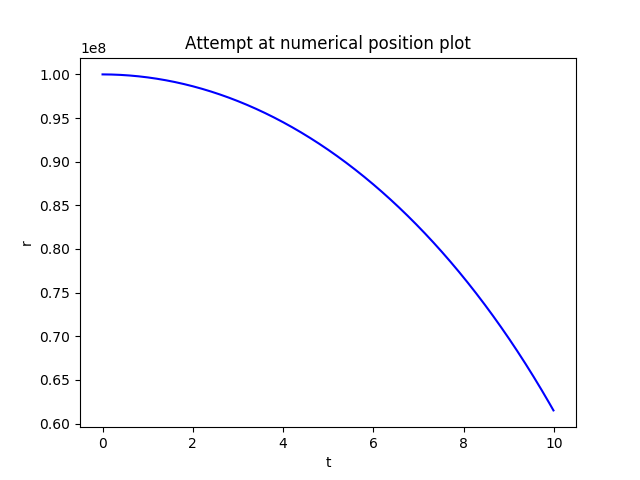
\includegraphics[scale=0.8]{attempt.png}
\end{figure} 






f. \textbf{Confirm Kepler's Second and Third Laws using your numerical solutions. Note that since the Second Law is equivalent to angular momentum conservation, its confirmation reduces to confirming angular momentum conservation. To confirm the 3rd law, determine the time period $T$ and the semi-major axis $a$ of the ellipse $a$ for each numerically obtained orbit. Then, plot $\log T$ versus $\log a$ for various initial conditions. What should the slope be? Verify that the plot has the correct slope using linear regression.} \\



I cannot confirm Kepler's Second and Third Laws because my numerical solutions didn't work out. However, I do know Kepler's Third Law, which is that the oribital period of  a planet is proportional to the semi-major axis of its orbit. $P$ is the orbital period, and $a$ is the semi-major axis, then the relationship is:

\begin{equation}
\frac{P^2}{a^3}
\end{equation}

This can be simplified to a constant, since $m$, the planet's mass, is insignificant when compared to a mass like the Sun, $M$:

\begin{equation}
\frac{4\pi}{G(M+m)} \approx \frac{4\pi}{G(M)}
\end{equation}

I would expect the slope of the log plot to be this constant. \\

Short Bibliography:

Classical Dynamics of Particles and Systems, by Thornton and Marion


\end{homeworkProblem}
\clearpage

%----------------------------------------------------------------------------------------

\end{document}